% -*- coding: UTF-8 -*-
% vim: autoindent expandtab tabstop=4 sw=4 sts=4 filetype=tex
% vim: spelllang=de spell
% chktex-file 27 - disable warning about missing include files

\subsection{Sphere Tracing}
\label{subsec:sphere_tracing}

Das von~\citeauthor{hart_sphere_1994} vorgeschlagene Sphere Tracing
Verfahren ist ein~\hyperref[subsec:ray_tracing]{Ray Tracing} Verfahren
für~\hyperref[subsec:implicit_surfaces]{implizite Oberflächen}. Es ist
ebenfalls ein~\hyperref[subsec:ray_marching]{Ray Marching} Verfahren.
Jedoch wird die Distanz der Abtastungsschritte eines (Licht-) Strahles
aufgrund einer~\hyperref[ssubsec:distance_functions]{Distanzfunktion}
bestimmt.
Das Verfahren wurde erstmalig~\citeyear{hart_ray_1989}
in~\citetitle{hart_ray_1989} von~\citeauthor{hart_ray_1989}
vorgestellt~\parencite{hart_ray_1989}.

Ein möglicher Algorithmus, wie Sphere Tracing umgesetzt werden kann,
findet sich in~\autoref{alg:sphere_tracing}.

Bei Sphere Tracing werden die Schnittpunkte eines (Licht-) Strahles
durch eine Folge von negativen Hüllkörpern (``unbounding volumes'') ---
bzw.\ in diesem Fall Kugeln (``unbounding spheres'') --- beschrieben.
Davon kommt die Bezeichnung Sphere Tracing~\parencite[S.
530]{hart_sphere_1994}.

``Unbounding volumes'' (zu Deutsch etwa ``negativer Hüllkörper'') wird
von den Autoren~\citeauthor{hart_ray_1989} benutzt, um das Sphere
Tracing Verfahren zu beschreiben und darzustellen. Der Term steht im
Gegensatz zu dem gängigen Konzept des Hüllkörpers (``bounding volume'').
Bei einem Hüllkörper wird ein Körper umschlossen. Der ``negative
Hüllkörper'' umschliesst ein Stück des Raumes ohne dabei ein Objekt zu
umschliessen (dass heisst ohne ein gesuchtes Objekt zu
``berühren'')~\parencite[S. 291]{hart_ray_1989}. Die ``negativen
Hüllkörper'' sind in~\autoref{fig:sphere_tracing_1} als Kreisflächen
dargestellt.

Für die Berechnung eines negativen Hüllkörpers sucht man
den Abstand eines Objektes von einem Ausgangspunkt.
Ist die kürzeste Distanz zwischen Ausgangspunkt und
Objekt bekannt, kann diese als Radius einer Kugel angenommen werden. 

Objekte sind bei dem genannten Verfahren durch Distanzfunktionen
definiert. So ist z.B. eine Kugel als Punkt im Raum minus deren Radius
definiert (siehe~\autoref{eq:surface_immplicit_geometric}). Der
Betrachter kann dabei auch als Punkt im Raum angenommen werden. Somit
sind alle Distanzen bekannt (siehe auch
Distanzfelder,~\autoref{ssubsec:distance_fields}).

Eine Kugel dient als negativer Hüllkörper (``unbounding Volume''). Sie
ist aber \textit{nicht} Teil des Objektes und schneidet dieses
auch nicht (ist also nicht $\overset{\circ}{\bm{A}}$).\\
Nur der äusserste Punkt des Abstandes  liegt genau
auf der Oberfläche des Objektes ($\partial \bm{A}$). Der Radius einer
solchen Kugel wird durch Evaluation der Distanzfunktion eines
abzutastenden Punktes im Raum bestimmt.

\citeauthor{hart_ray_1989} beschreiben in ihrer
Arbeit~\citetitle{hart_ray_1989} die Darstellung von Fraktalen im
dreidimensionalen Raum. Es wird von einer Abschätzung der Distanz
gesprochen, da diese für Fraktale nicht effizient berechnet werden
kann~\parencite[S.  291]{hart_ray_1989}.\\
Bei ``regulären'' Objekten, wie z.B. einer Kugel, kann der zur
Oberfläche am nächsten gelegene Punkt von einem beliebigen Punkt
derselben Domäne exakt berechnet werden~\parencite[S.
530]{hart_sphere_1994}. Dies ist durch die
implizite~\autoref{eq:surface_implicit_sphere} gegeben.

Gemäss~\cite[S. 291 - 292]{hart_ray_1989} geschieht die Verfolgung der
Strahlen bei Sphere Tracing wie folgt: Ein Strahl wird vom Betrachter
(Auge bzw.  Lochkamera) durch die Bildebene zu einem Objekt geschossen.
Dabei wird bei dem initialen Ausgangspunkt der Radius eines negativen
Hüllkörpers in Form einer ersten Kugel berechnet, so wie oben beschrieben.
Dies ist die Distanz, welche der Strahl in einem ersten
Schritt effektiv zurücklegen wird. Von diesem Schnittpunkt aus wird
erneut der Radius einer Kugel berechnet usw.

Dies geschieht so lange, bis der Strahl schliesslich von einem
Schnittpunkt des negativen Hüllkörpers aus auf die Oberfläche eines
Objektes trifft.\\
Ein weiteres Kriterium für den Abbruch ist eine vordefinierte maximale
Distanz des Strahles ($d_{\text{max}}$). Ist diese erreicht und der
Strahl verfehlt die Oberfläche des Objektes, wird abgebrochen. Somit ist
auch ersichtlich, dass Sphere Tracing nicht die genannten Problematiken
von Ray Marching aufweist (siehe~\autoref{subsec:ray_marching}).

Die folgenden Abbildungen~\ref{fig:sphere_tracing_1}
und~\ref{fig:sphere_tracing_2} veranschaulichen das Sphere Tracing
Verfahren.

\begin{figure}[H]
    \centering
    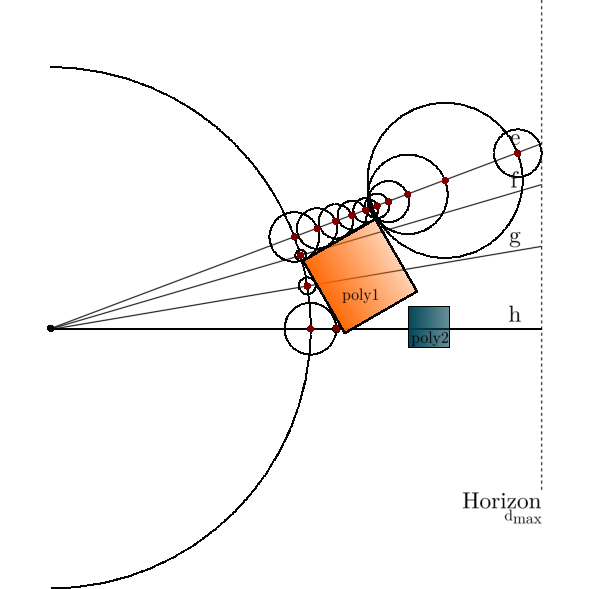
\includegraphics{img/sphere_tracing_principle.pdf}
    \caption{Illustration des Sphere Tracing
        Verfahrens.\protect\footnotemark}\label{fig:sphere_tracing_1}
\end{figure}
\footnotetext{Eigene Darstellung mittels Inkscape.}

\begin{figure}[H]
    \centering
    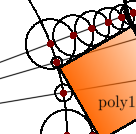
\includegraphics[width=0.5\textwidth]{img/sphere_tracing_principle_near.pdf}
    \caption{Illustration des Sphere Tracing Verfahrens,
        Nahaufnahme.\protect\footnotemark}\label{fig:sphere_tracing_2}
\end{figure}
\footnotetext{Eigene Darstellung mittels Inkscape.}

Ausgehend von der parametrischen Beschreibung eines (Licht-) Strahles
(\autoref{eq:ray_param}), beschreiben~\citeauthor{hart_ray_1989} die
Richtung $r_{d}$ eines Strahles als Einheitsvektor~\parencite[S.
291]{hart_ray_1989}:

\begin{gather}
    r_{d} = \frac{p_{x, y} - r_{0}}{|p_{x, y} - r_{0}|}
\end{gather}

wobei $r_{0}$ der Ursprung eines Strahles und $p_{x, y}$ ein Punkt der Bildebene ist.

Um nun den Schnittpunkt eines Strahles $r_{d}$ mit der Oberfläche eines
Objektes zu finden, muss~\autoref{eq:ray_param_cond}, $F(t) = f \circ
r = 0$, gelöst werden. Dabei ist --- wie oben definiert --- die Funktion
$f(x)$ nun eine Distanzfunktion, wie zum Beispiel die geometrische
Distanzfunktion zur Beschreibung einer Kugel
(Gleichung~\ref{eq:surface_immplicit_geometric}).

Evaluiert man nun die Gleichung $F(t)$ unter Anwendung der eben beschriebenen
Verfolgung der Strahlen, findet man so die erste positive Nullstelle der Gleichung
$F(t)$. Diese Nullstelle ist die Grenze der Folge von negativen Hüllkörpern
(``unbounding spheres''), welche durch die rekursive Gleichung:

\begin{gather}
    t_{i+1} = t_{i} + F(t_{i})
\end{gather}

definiert ist. Der Ursprungspunkt ist dabei als $t_{0}$ definiert. Diese Folge
konvergiert genau dann --- und nur dann --- wenn der Strahl auf die implizite
Oberfläche eines Objektes trifft. Diese Folge bildet den Kern des Algorithmus
zur Darstellung von geometrisch definierten, impliziten Oberflächen.

\begin{lstlisting}[language=Python,caption={Eine abstrakte Umsetzung des Sphere
        Tracings\protect\footnotemark.},label={alg:sphere_tracing},captionpos=b,emph={sphere_trace}]
def sphere_trace():
    ray_distance          = 0
    estimated_distance    = 0
    max_distance          = 9001
    convergence_precision = 0.000001

    while ray_distance < max_distance:
        # sd_sphere is a signed distance function defining the implicit surface
        # cast_ray defines the ray equation given the current travelled /
        # marched distance of the ray
        estimated_distance = sd_sphere(cast_ray(ray_distance))

        if estimated_distance < convergence_precision:
            # the estimated distance is already smaller than the desired
            # precision of the convergence, so return the distance the ray has
            # travelled as we have an intersection
            return ray_distance

        ray_distance = ray_distance + estimated_distance

    # When we reach this point, there was no intersection between the ray and a
    # implicit surface, so simply return 0
    return 0
\end{lstlisting}
\footnotetext{Algorithmus in Pseudocode gemäss~\cite{hart_sphere_1994}[S. 531,
    Fig. 1]}
